% Exact randomized revealing-optimization curve.
\begingroup
\tracinglostchars=0
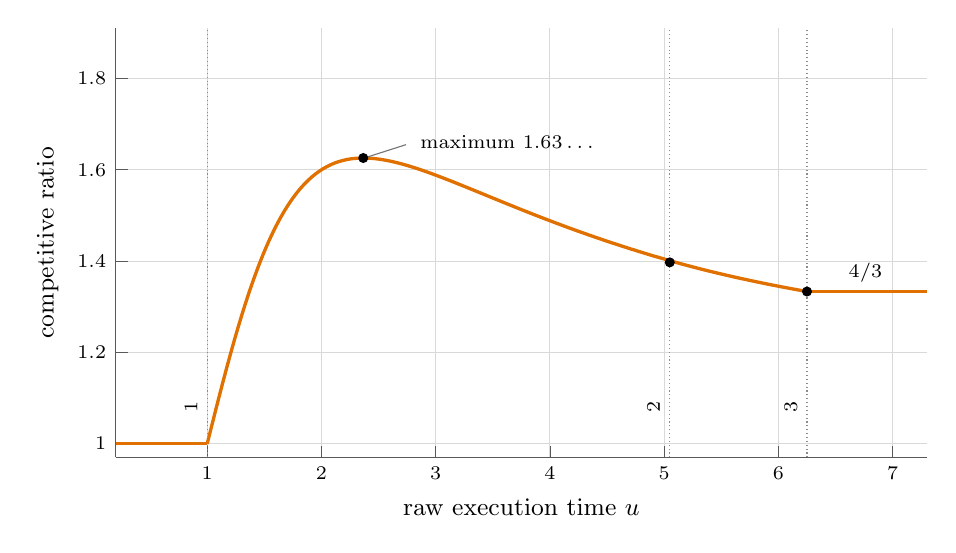
\begin{tikzpicture}
\begin{axis}[
  width=0.98\linewidth,
  height=0.58\linewidth,
  xmin=0.2,
  xmax=7.3,
  ymin=0.97,
  ymax=1.91,
  xlabel={raw execution time $u$},
  ylabel={competitive ratio},
  xtick={1,2,3,4,5,6,7},
  ytick={1,1.2,1.4,1.6,1.8},
  tick label style={font=\scriptsize},
  label style={font=\small},
  grid=major,
  grid style={black!15},
  axis line style={black!65},
  tick style={black!65},
  axis x line*=bottom,
  axis y line*=left,
  samples=120,
  no markers,
  clip=true,
]

\addplot[orange!88!black,very thick,domain=0.2:1] {1};
\addplot[orange!88!black,very thick,domain=1:5.04891733952]
  {x^3/(x^2+(x-1)^3)};
\addplot[orange!88!black,very thick,domain=5.04891733952:6.25]
  {1+1/(2*(sqrt(x)-1))};
\addplot[orange!88!black,very thick,domain=6.25:7.3] {4/3};
\addplot[black!45,densely dotted,thin] coordinates {(1,0.97) (1,1.91)};
\node[font=\scriptsize,rotate=90,anchor=south]
  at (axis cs:1,1.08) {$\uRand{1}$};
\addplot[black!45,densely dotted,thin]
  coordinates {(5.04891733952,0.97) (5.04891733952,1.91)};
\node[font=\scriptsize,rotate=90,anchor=south]
  at (axis cs:5.04891733952,1.08) {$\uRand{2}$};
\addplot[black!45,densely dotted,thin]
  coordinates {(6.25,0.97) (6.25,1.91)};
\node[font=\scriptsize,rotate=90,anchor=south]
  at (axis cs:6.25,1.08) {$\uRand{3}$};
\addplot[only marks,mark=*,mark size=1.6pt,black] coordinates {
  (2.36602540378,1.62575238458)
  (5.04891733952,1.39719767662)
  (6.25,1.33333333333)
};
\node[font=\scriptsize,anchor=west] at (axis cs:2.78,1.66)
  {maximum $1.63\ldots$};
\draw[black!55,thin] (axis cs:2.74,1.655) -- (axis cs:2.39,1.627);
\node[font=\scriptsize,anchor=west] at (axis cs:6.53,1.375) {$4/3$};

\end{axis}
\end{tikzpicture}
\endgroup
